\documentclass[10pt,aspectratio=169,serif]{beamer}

\usepackage[fontset=none, scheme=plain]{ctex}
\IfFontExistsTF{Songti SC}{%
	\setCJKmainfont{Songti SC}[AutoFakeSlant=0.2]%
	\setCJKsansfont{Songti SC}[AutoFakeSlant=0.2]%
}{%
	\setCJKmainfont{FandolSong-Regular}[Extension=.otf,BoldFont=FandolSong-Bold,AutoFakeSlant=0.2]%
	\setCJKsansfont{FandolSong-Regular}[Extension=.otf,BoldFont=FandolSong-Bold]%
}
\usepackage{amsmath,amssymb,graphicx,tikz,booktabs,multicol,calligra}
\usepackage{pgfplots}
\pgfplotsset{compat=1.18}
\usepackage{tcolorbox}
\tcbuselibrary{skins}
\usepackage{XyygU}
\usepackage{caption}
\captionsetup[figure]{name=图,labelsep=period}

\usetikzlibrary{arrows.meta,positioning,calc}

\setlength{\abovedisplayskip}{0pt plus 2pt minus 2pt}
\setlength{\belowdisplayskip}{0pt plus 2pt minus 2pt}

\title[单调性与最值练习]{3.2.1 单调性与最大（小）值（练习）}
\subtitle{定义证明 \& 图象 \& 最值}
\author{}
\institute{}
\date{2026-10-16}

\begin{document}

\begin{frame}
  \titlepage
\end{frame}

% ========== 第1题 ==========
\begin{frame}[t]{第1题：由图象描述变化规律}
\textbf{1.} 请根据下图描述某装配线的生产效率与生产线上工人数量间的关系。

\vspace{0.5em}
\begin{center}
\begin{tikzpicture}[scale=1.1]
\begin{axis}[
    width=8cm, height=5cm,
    axis lines=middle,
    xlabel={工人数}, ylabel={生产效率},
    xmin=-1, xmax=10, ymin=-1, ymax=4,
    xtick=\empty, ytick=\empty,
    xlabel style={below},ylabel style={right},
]
\draw[thick,magenta] (0,0) parabola bend (5,3.5)  (8,2);
\node[below left] at (0,0) {$O$};
%\addplot[thick,magenta,domain=0:9,samples=100] {0.6*sin(deg(x*40))*exp(-0.05*x)+0.5*x*exp(-0.15*x)};
\end{axis}
\end{tikzpicture}
\end{center}
\end{frame}

\begin{frame}[t]{第1题 解答}
\begin{tcolorbox}[colback=orange!10,colframe=orange,title=\textbf{解}]
随着生产线上工人数量的增加：

\vspace{0.3em}
\begin{itemize}
  \item 在工人数量较少时，生产效率随工人数量增加而 \alert{逐渐上升}；
  \item 当工人数量达到某个值时，生产效率达到 \alert{最大值}；
  \item 工人数量继续增加，生产效率反而 \alert{逐渐下降}（人浮于事、相互等待）。
\end{itemize}

\vspace{0.3em}
即：生产效率关于工人数的函数先单调递增，达到峰值后单调递减。
\end{tcolorbox}
\end{frame}

% ========== 第2题 ==========
\begin{frame}[t]{第2题：证明一次函数是增函数}
\textbf{2.} 根据定义证明函数 $f(x)=3x+2$ 是增函数。
\end{frame}

\begin{frame}[t]{第2题 解答}
\begin{tcolorbox}[colback=orange!10,colframe=orange,title=\textbf{证明}]
任取 $x_1,\,x_2\in\mathbf{R}$，且 $x_1<x_2$。

\vspace{0.3em}
作差：
\[
f(x_1)-f(x_2)=(3x_1+2)-(3x_2+2)=3(x_1-x_2).
\]

\vspace{0.3em}
因为 $x_1<x_2$，所以 $x_1-x_2<0$，从而
\[
f(x_1)-f(x_2)=3(x_1-x_2)<0,
\]
即 $f(x_1)<f(x_2)$。

\vspace{0.3em}
所以 $f(x)=3x+2$ 在 $\mathbf{R}$ 上是 \alert{增函数}。
\end{tcolorbox}
\end{frame}

% ========== 第3题 ==========
\begin{frame}[t]{第3题：证明反比例函数的单调性}
\textbf{3.} 证明函数 $\displaystyle f(x)=-\frac{2}{x}$ 在区间 $(-\infty,0)$ 上单调递增。
\end{frame}

\begin{frame}[t]{第3题 解答}\vspace{-1em}
\begin{tcolorbox}[colback=orange!10,colframe=orange,title=\textbf{证明}]
任取 $x_1,\,x_2\in(-\infty,0)$，且 $x_1<x_2$。

\vspace{0.3em}
作差：
\[
f(x_1)-f(x_2)=\left(-\frac{2}{x_1}\right)-\left(-\frac{2}{x_2}\right)
=\frac{2}{x_2}-\frac{2}{x_1}
=\frac{2(x_1-x_2)}{x_1x_2}.
\]

\vspace{0.3em}
因为 $x_1<x_2<0$，所以 $x_1-x_2<0$，且 $x_1x_2>0$，于是
\[
f(x_1)-f(x_2)=\frac{2(x_1-x_2)}{x_1x_2}<0,
\]
即 $f(x_1)<f(x_2)$。

\vspace{0.3em}
所以 $f(x)=-\dfrac{2}{x}$ 在 $(-\infty,0)$ 上 \alert{单调递增}。
\end{tcolorbox}
\end{frame}

% ========== 第4题 ==========
\begin{frame}[t]{第4题：反比例函数的定义域与单调性}
\textbf{4.} 画出反比例函数 $\displaystyle y=\frac{k}{x}$ 的图象。

\vspace{0.8em}
(1) 这个函数的定义域 $D$ 是什么？

\vspace{0.8em}
(2) 它在定义域 $D$ 上的单调性是怎样的？证明你的结论。
\end{frame}

\begin{frame}[t]{第4题 图象（以 $k>0$ 为例）}
\begin{center}
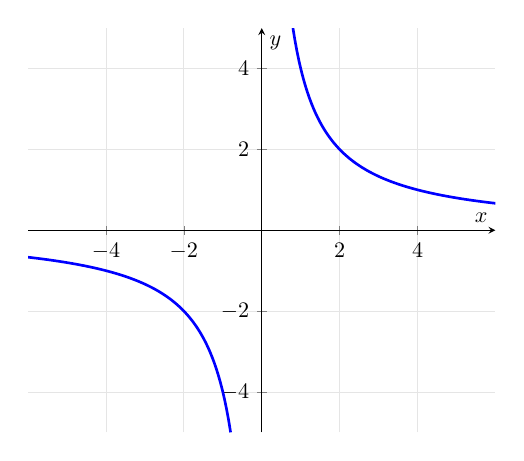
\begin{tikzpicture}[scale=0.8]
\begin{axis}[
    width=9cm, height=8cm,
    axis lines=middle,
    xlabel=$x$, ylabel=$y$,
    xmin=-6, xmax=6, ymin=-5, ymax=5,
    xtick={-4,-2,2,4}, ytick={-4,-2,2,4},
    grid=major, grid style={gray!20},
]
\addplot[very thick,blue,domain=-6:-0.8,samples=100] {4/x};
\addplot[very thick,blue,domain=0.8:6,samples=100] {4/x};
\end{axis}
\end{tikzpicture}
\end{center}
\end{frame}

\begin{frame}[t]{第4题 解答}
\begin{tcolorbox}[colback=orange!10,colframe=orange,title=\textbf{解}]
(1) 定义域 $D=(-\infty,0)\cup(0,+\infty)$。

\vspace{0.3em}
(2) 以 $k>0$ 为例（$k<0$ 同理）：

任取 $x_1<x_2<0$，
\[
f(x_1)-f(x_2)=\frac{k}{x_1}-\frac{k}{x_2}=\frac{k(x_2-x_1)}{x_1x_2}.
\]
因为 $x_1x_2>0$，$x_2-x_1>0$，$k>0$，所以 $f(x_1)-f(x_2)>0$，即 $f(x_1)>f(x_2)$。

\vspace{0.3em}
故 $y=\dfrac{k}{x}$ 在 $(-\infty,0)$ 上 \alert{单调递减}；同理在 $(0,+\infty)$ 上也 \alert{单调递减}。

\vspace{0.3em}
\small（注意：不能说它在整个定义域上单调递减，因为 $x_1=-1,\ x_2=1$ 时 $f(-1)=-k<k=f(1)$，并不递减。）
\end{tcolorbox}
\end{frame}

% ========== 第5题 ==========
\begin{frame}[t]{第5题：气温变化的图象与单调区间}
\textbf{5.} 整个上午（8:00$\sim$12:00）天气越来越暖，中午时分（12:00$\sim$13:00）一场暴风雨使天气骤然凉爽了许多。暴风雨过后，天气转暖，直到太阳落山（18:00）才又开始转凉。画出这一天 8:00$\sim$20:00 期间气温作为时间函数的一个可能的图象（示意图），并说出所画函数的单调区间。
\end{frame}

\begin{frame}[t]{第5题 图象与解答}
\begin{center}
\begin{tikzpicture}[scale=0.75]
\begin{axis}[
    width=11cm, height=5.5cm,
    axis lines=middle,
    xlabel={时刻}, ylabel={气温},
    xmin=8, xmax=20, ymin=0, ymax=40,
    xtick={8,12,13,18,20},
    xticklabels={8,12,13,18,20},
    ytick=\empty,
    grid=major, grid style={gray!20},
]
\addplot[thick,red,domain=8:12,samples=50] {10+1.5*(x-8)};
\addplot[thick,red,domain=12:13,samples=50] {16-8*(x-12)};
\addplot[thick,red,domain=13:18,samples=50] {8+1.2*(x-13)};
\addplot[thick,red,domain=18:20,samples=50] {14-2*(x-18)};
\end{axis}
\end{tikzpicture}
\end{center}
\begin{tcolorbox}[colback=orange!10,colframe=orange,title=\textbf{单调区间}]
单调递增：$[8,12]$，$[13,18]$；\quad 单调递减：$[12,13]$，$[18,20]$。
\end{tcolorbox}
\end{frame}

% ========== 第6题 ==========
\begin{frame}[t]{第6题：由单调区间画图象}
\textbf{6.} 设函数 $f(x)$ 的定义域为 $[-6,11]$。如果 $f(x)$ 在区间 $[-6,-2]$ 上单调递减，在区间 $[-2,11]$ 上单调递增，画出 $f(x)$ 的一个大致的图象，从图象上可以发现 $f(-2)$ 是函数 $f(x)$ 的一个 \underline{\hspace{3cm}}。
\end{frame}

\begin{frame}[t]{第6题 解答}
\begin{center}
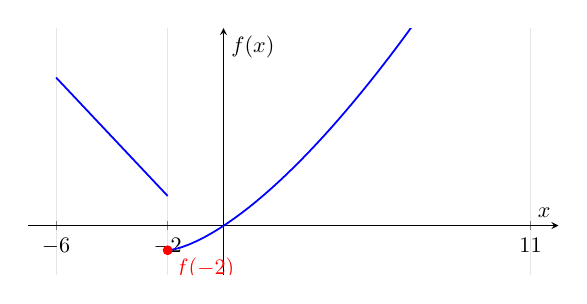
\begin{tikzpicture}[scale=0.8]
\begin{axis}[
    width=10cm, height=5.5cm,
    axis lines=middle,
    xlabel=$x$, ylabel=$f(x)$,
    xmin=-7, xmax=12, ymin=-2, ymax=8,
    xtick={-6,-2,11},
    ytick=\empty,
    grid=major, grid style={gray!20},
]
\addplot[thick,blue,domain=-6:-2,samples=50] {6-1.2*(x+6)};
\addplot[thick,blue,domain=-2:11,samples=50] {-1+0.35*(x+2)^1.5};
\addplot[only marks,mark=*,mark size=2pt,red] coordinates {(-2,-1)};
\node[red,below right] at (axis cs:-2,-1) {$f(-2)$};
\end{axis}
\end{tikzpicture}
\end{center}
\begin{tcolorbox}[colback=orange!10,colframe=orange,title=\textbf{结论}]
$f(-2)$ 是函数 $f(x)$ 的一个 \alert{最小值}。
\end{tcolorbox}
\end{frame}

% ========== 第7题 ==========
\begin{frame}[t]{第7题：求闭区间上的最值}
\textbf{7.} 已知函数 $\displaystyle f(x)=\frac{1}{x}$，求函数在区间 $[2,6]$ 上的最大值和最小值。
\end{frame}

\begin{frame}[t]{第7题 解答}
\begin{tcolorbox}[colback=orange!10,colframe=orange,title=\textbf{解}]
先证明 $f(x)=\dfrac{1}{x}$ 在 $[2,6]$ 上单调递减。

任取 $x_1,x_2\in[2,6]$，$x_1<x_2$：
\[
f(x_1)-f(x_2)=\frac{1}{x_1}-\frac{1}{x_2}=\frac{x_2-x_1}{x_1x_2}>0,
\]
故 $f(x_1)>f(x_2)$，$f(x)$ 在 $[2,6]$ 上单调递减。

\vspace{0.3em}
因此在端点处取最值：
\[
f_{\max}=f(2)=\frac{1}{2},\qquad f_{\min}=f(6)=\frac{1}{6}.
\]
\end{tcolorbox}
\end{frame}

\begin{frame}[c]
  \begin{center}
    {\Huge\calligra Thanks!}
  \end{center}
\end{frame}

\end{document}
